\infolevone{
\section[Target Chamber]{Target Chamber
\label{sec:target_chamb}
%\footnote{
}
%  $CVS~revision~ $Id: tgtcham.tex,v 1.11 2005/04/04 22:27:25 gen Exp $ $
%}
%\footnote{Authors: ?? \email{??@jlab.org}}

%Need to replace with Hall C target chamber info.  (Or subsum in targets chapter)

The cryotargets and the associated solid targets 
(see Sec.~\ref{sec:targets-overv}) 
are contained in a special target chamber consisting of a large evacuated  cylinder in two stacked sections. 

The chamber was designed (in 2006) to isolate the beam line vacuum from  each
spectrometer so that each could rotate
around the target without vacuum coupling and without jeopardizing
the  kinematics and acceptance specified
 for approved experiments at that time.  It was also designed to simultaneously
 contain a liquid or gas target and an array of conductively cooled solid targets hung below the cryo-targets. A single axis (vertical) motion system is employed to select the desired target.
The desired kinematic specifications that were
 considered included momentum and energy resolution in both arms,
 angular range of spectrometers, angular acceptance, and luminosity. The relevant JLab drawing numbers are 67153-E-56001 to 67153-E-56020, although as described below, the window design has changed dramatically. Note that the portal to JLab drawings is \url{https://misportal.jlab.org/jlabDocs/search.seam}.
 
The chamber vacuum is isolated from the atmosphere by a thin aluminum window. The nominal vacuum is typically a few times $10^{-6}$ Torr warm, and about a decade less with a cold cryotarget. Operation with the scattering chamber vacuum in or even near the $10^{-4}$ Torr range is not recommended. 

\subsection{Vacuum Window}
The scattering chamber can be configured differently (in principle) for different experiments by having different window configurations and rotations of the scattering chamber about its central vertical axis. The nominally 2 inch thick aluminum chamber has an inner diameter of 41 inches, and an outer diameter of 45 inches, not including the semi-cylindrical window flanges or extruding ports. In the standard configuration (see Fig.~\ref{fig:SC_Window_CAD}), both spectrometers share a single ``smile'' (cut-out) on the scattering chamber. The exit beam pipe connects via a threaded compression flange (no o-ring) to this scattering chamber window. A conflat-style seal is employed using an Iconel 718 seal. An aluminum nut on the evacuated side of the window seals the window to the aluminum compression flange, as detailed in drawing 67153-56029. The 2024-T3 aluminum hydro-formed window is 0.020 $in$ thick. The window surface is relatively smooth, with mild wrinkles from the hydro-formed design. The window design (see Fig.~\ref{Window_Photo}) supports the exit beam pipe flange in a novel way in order to keep o-rings far (\textgreater 7.5 $in$) from the beamline, which should mitigate problems with radiation damage and subsequent vacuum leaks which plagued the old design. 

The new design also greatly reduces the mass next to the beam axis at the scattering chamber exit.  
%The exit beam pipe is supported mechanically by a pair of struts that attach to the window frame, with the design goal to minimize the amount of material close to the beam axis. 
The mass associated with the 2 $in$ thick chamber wall and window frames near the beam axis is essentially replaced as a source of background by the thinner compression flange/nut on the window, which furthermore subtends a much smaller solid angle from the target than the old arrangement did. The minimum scattering angle from the target center which does not interfere with the exit beam pipe flange is 3.2$^\circ$.

\begin{figure}[!htb]
%\vspace*{-1.8cm}
\begin{center}
%\hspace*{0.5cm}
%\includegraphics[width =0.95\textwidth,angle=-90]{Pics/QWEAK-tgt-schematic.pdf}
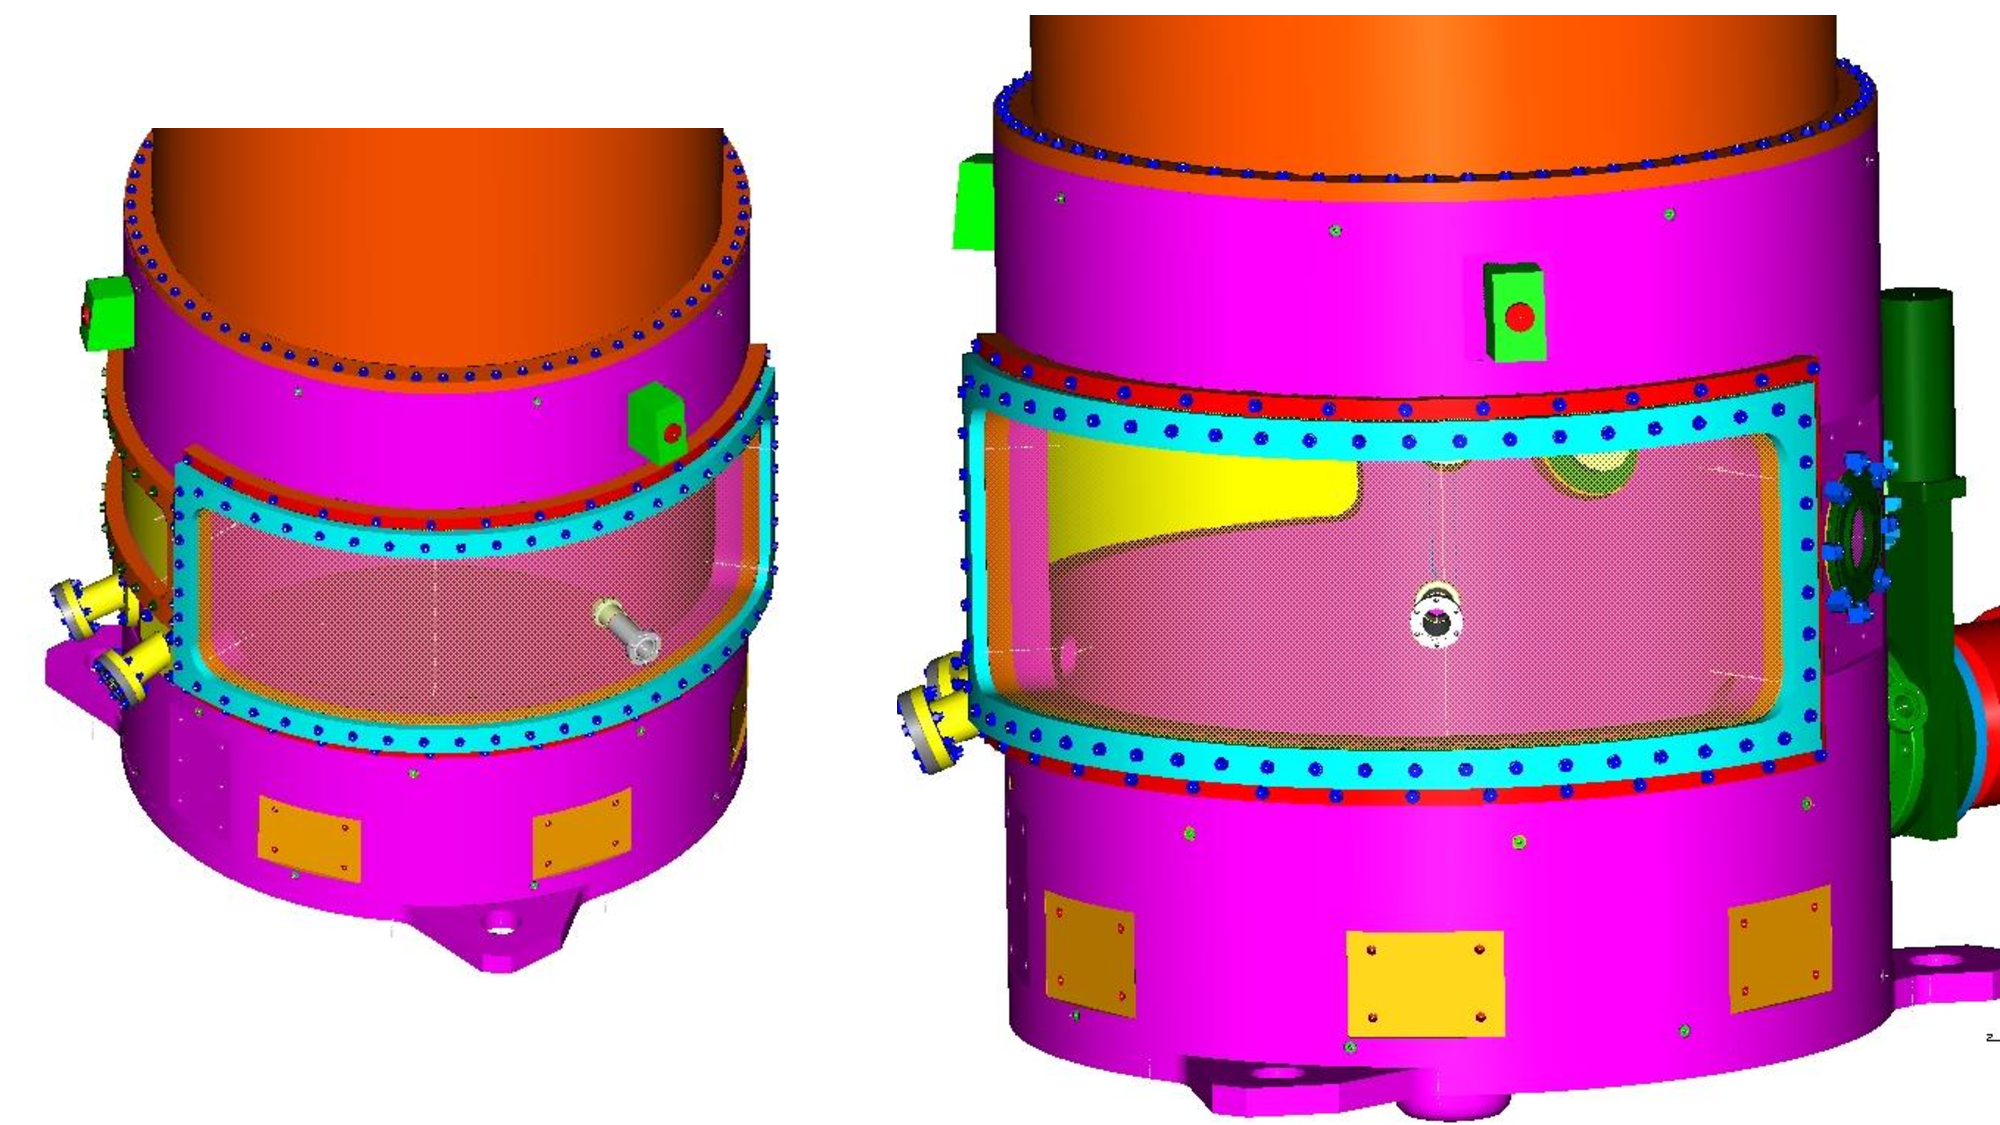
\includegraphics[width =1.0\textwidth]{SC_Window_CAD2.pdf}
\end{center}
%\vspace*{0.5cm}
\caption[tgt-layout]{ A couple CAD drawings showing some details of the new scattering chamber window design. The exit beam pipe is shown protruding from the window. The SHMS opening is on the right side of the picture; the HMS opening is on the left side. The turbopump and its gate valve are visible on the extreme right.}
\label{fig:SC_Window_CAD}
\end{figure}

\begin{figure}[!htb]
%\vspace*{-1.8cm}
\begin{center}
\hspace*{-3.5cm}
%\includegraphics[width =0.95\textwidth,angle=-90]{Pics/QWEAK-tgt-schematic.pdf}
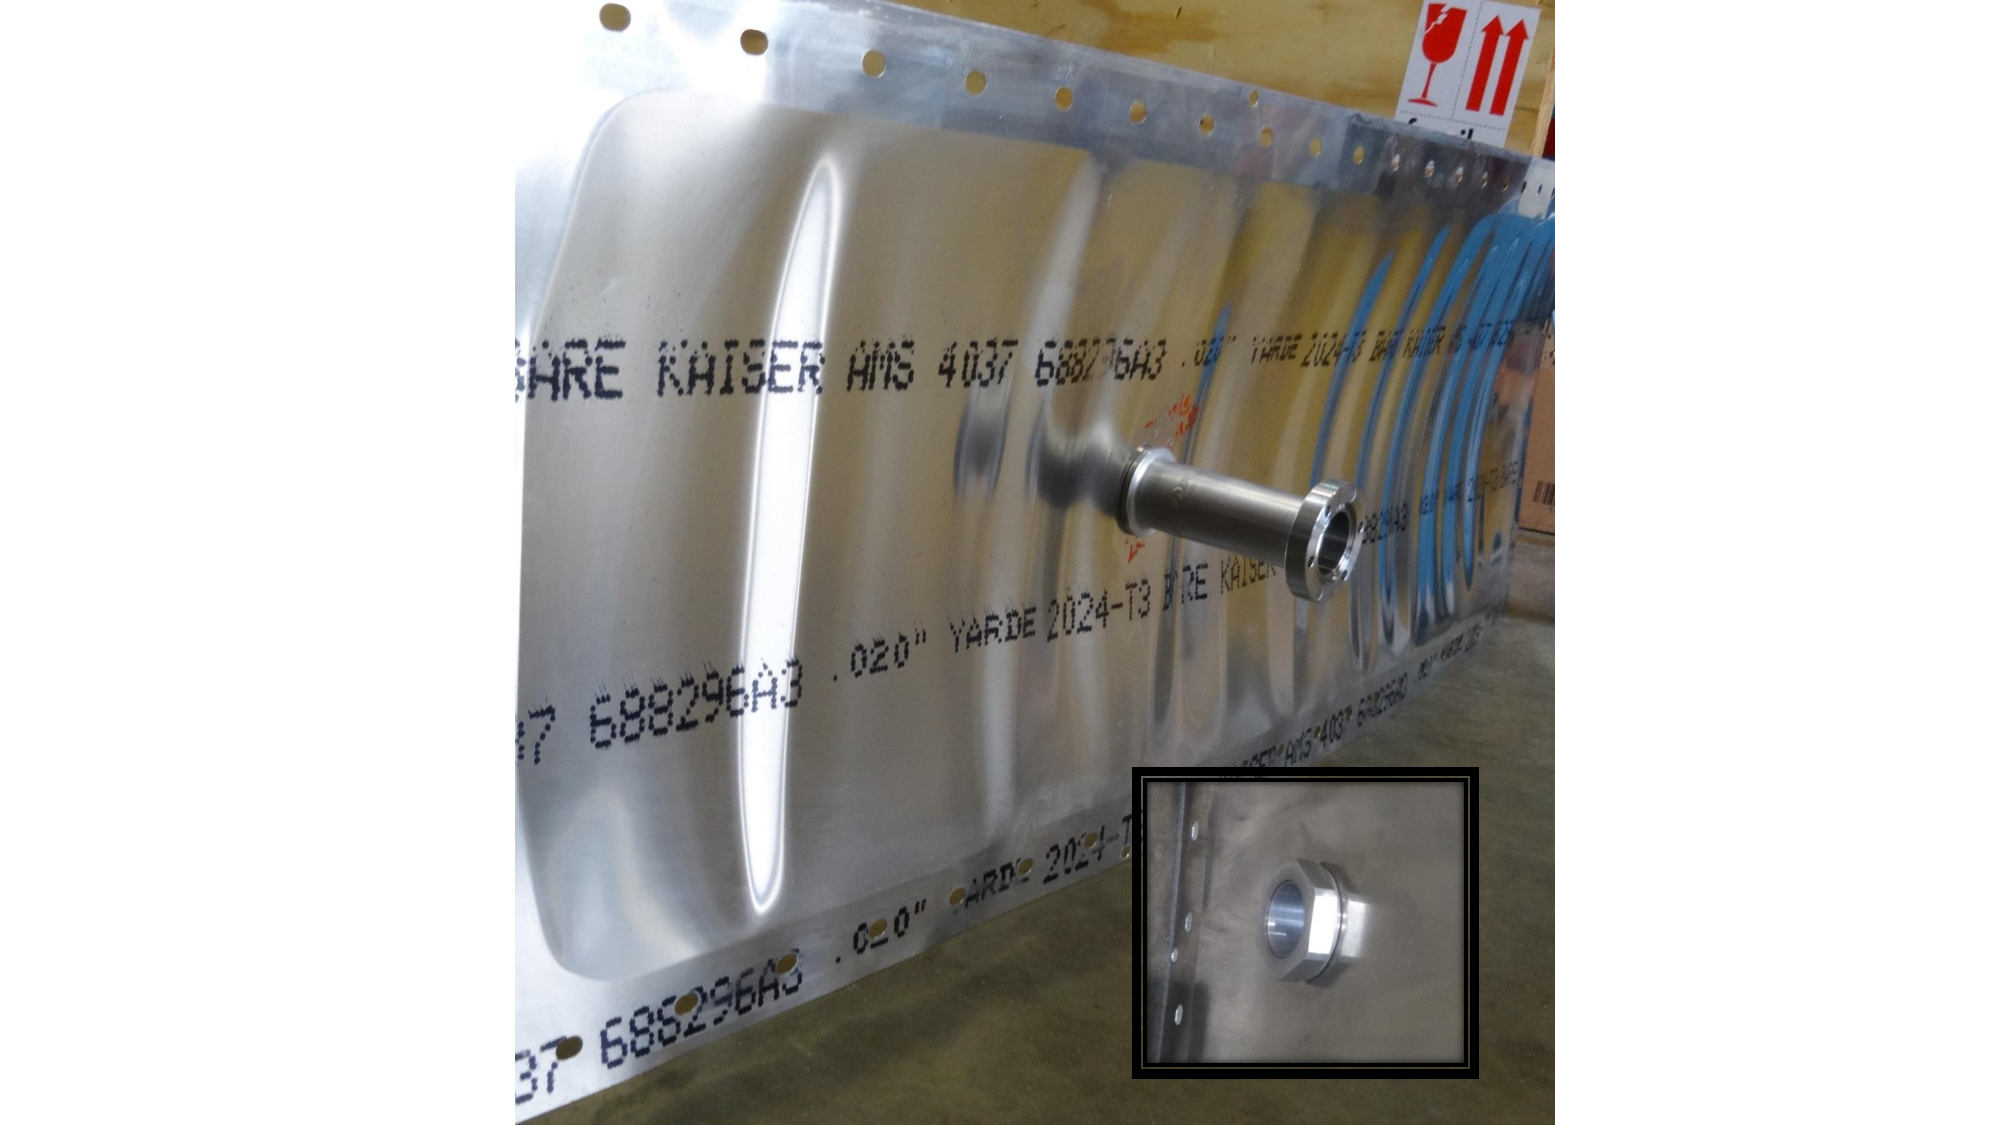
\includegraphics[width =1.5\textwidth]{Window_Photo.pdf}
\end{center}
%\vspace*{0.5cm}
\caption[tgt-layout]{\label{Window_Photo} Photograph of the scattering chamber window with the short exit beam pipe attached. The inset shows the nut on the opposite side (the vacuum side) attaching this beam pipe to the window.}
\end{figure}

\subsection{Angle Ranges}
On the HMS side, the horizontal angular range is from 3.2 to 77.0 degrees, and $\pm 17.3 ^\circ$ vertically. On the SHMS side, the horizontal angular range is 3.2$^\circ$ to 47.0$^\circ$ degrees, and $\pm 17.3 ^\circ$ vertically.  The angular limits presented by the scattering chamber are less restrictive than the limits associated with the spectrometers themselves. The SHMS can be moved over the angular range from 5.5 to 40 degrees, and the HMS can be rotated from 10.5$^\circ$ out to about 80$^\circ$. The minimum opening angle between the two spectrometers is 17.5$^\circ$, or greater depending on the exit beam pipe in use.

\subsection{Penetrations}

There are also openings in the scattering chamber through which the beam
can enter, two pumping ports, several viewports, and
some spare ports. A remotely controlled TV camera and light are used in conjunction with the viewports to observe target motion and position in the counting room. Beam position on the target can be viewed even at low beam currents with a scintillating BeO target, or on the cryotarget cell window via transition radiation which produces a visible spot above 5 or 10 $\mu$A. 

Top and bottom plates complete the shell of the scattering chamber.
The bottom plate is mounted to an adjustment plate on the
solid shaft which forms the pivot axis for the two spectrometers. The scattering chamber's bottom plate has the shape of an inverted top hat. The ``hat'' penetrates into an opening in the center of the pivot, allowing more vertical motion and more solid targets to be hung off the bottom of the cryotarget assembly. The hat extends 5.25 inches below the bottom surface of the 1.5 inch thick bottom plate, and has an i.d. of 5 inches.

The top plate has a number of penetrations. The largest of these allows
the cryotarget coolant plumbing, wiring, and lifting mechanisms into the vacuum and is sealed by
a large diameter bellows. 

%There is also a three inch diameter tube through
%which the solid targets are inserted.
%The other three openings are capped by eight inch diameter aluminum
%conflats and currently have no specified function.


%The target chamber is designed so that
%each spectrometer will have continuous coverage in the standard tune from
%$\theta_{min}=$12.54$^\circ$ to $\theta_{max}=$165$^\circ$.
%The aluminum window is 6~$in$ high and 0.016~$in$ thick made of 5052 H34 aluminum foil.
%The foil forms regularly spaced vertical ridges when
%placed under load. The window had an inter-ridge
%spacing of 3 inches.
%If the window is treated as a collection
%of smaller rectangular windows which have the full vertical height
%of 6 inches and the inter-ridge spacing as a width,
%then stress formulas predict that the 0.016 $in$
%material would reach ultimate stress at a pressure higher than 35 PSID
%(for both over-pressure and under-pressure). 
%There is a gate valve between the 
%scattering chamber and the beam entrance (exit) 
%pipe. Both 
%valves will be closed automatically in the
%event that the chamber vacuum begins to rise and an FSD will be caused
%( this is done via a relay output of the scattering
%chamber vacuum gauge). If either valve is closed an FSD will result.

%The target chamber is supported by a 24 $in$ diameter pivot post
%secured in concrete, rising about 93.6 $in$ above the Hall A cement floor.
%The Hall A target chamber
%consists of an aluminum middle ring, a stainless steel base ring,
%each with a 41.0 $in$ inner diameter,
%and a stainless steel cylindrical top hat with 40 $in$ inner diameter
%to enclose the cryotarget and secure the cryogenic connections.

%When the scattering chamber is under vacuum, there is a potential
%danger of window rupture.
%The loud noise from the rupture could hurt
%one's ears if not protected. Therefore when the chamber is under vacuum,
%protective covers are optionally put on when practicable during controlled access. These must be taken off
%for data taking. 
%For restricted access, the protective covers are required
%to be on when the chamber is under vacuum. Before switching from controlled
%access to restricted access, the protective covers must be installed by designated Hall C technicians.
%Anytime that the scattering chamber
%is under vacuum, the pivot area is enclosed in a rope or tape barrier
%and a warning sign is posted.
%Hearing protection is required in the enclosed area. Access to the pivot area is also controlled through a %pivot access document which must be read and signed before the pivot area can be accessed.

%\infolevone{
%	The aluminum ring with an outer diameter of 45.0 $in$ and
%wall thickness 2.0 $in$  is necessary for a sturdy support structure and
%to permit machining of the outside surface to accommodate
%the flanges for fixed and sliding seals mounted on
%opposite sides of the ring that vacuum connect the chamber to each HRS.
%The height of the aluminum ring shown is 36.0 $in$, which is
%designed to accommodate the mounting flanges.
%The stainless steel base ring 
%is 11.50 $in$ in height with
%one pump-out 6 $in$ diameter port  and with
%seven 4 $in$ viewing and electrical feed-through ports.
%The base ring will also contain support mechanisms for the solid
%target ladder assembly, a rotisserie for collimating slits, radiators, and
%magnetic
%fingers for
%removing the solid target vacuum-lock can. The total height of the top
%ring, middle ring, and
%base ring is 93.81 $in$. This length is partly determined by our desire to
%include with the cryogenic extended target a solid target vertical ladder
%secured in an inverted hat through a hole in the base of the chamber.

%	The base ring includes an end plate through which the
%inverted hat will be adapted to fit into the large vertical pipe serving
%as the pivot post for the Hall A spectrometers.

%	The stainless steel cylindrical top hat  has
%40.0 $in$ inner diameter, and is 0.375 $in$ thick and
%46.31 $in$ high , which is necessary to permit the
%cryotarget to be withdrawn and to make space available to expose the solid
%targets to the electron beam.

 %  The 200 $\mu$A electron beam, focused to a $\sim$\(0.1\, mm\times
%0.1\) mm spot and rastered $\pm$5 mm horizontally or vertically on the
%target, enters through a oval hole in the middle ring which
%is 2.06 $in$ wide and exits through a 1.81 $in$ hole connected to the
%exit pipe.
%}

%\infolevone{
%\subsection{Target Chamber - Spectrometer Coupling}

%   The aluminum middle ring will support a flange on each side for each high
%resolution spectrometer. Four flanges will be available: Two flanges will
%contain a 6 $in$ window opening which will be covered with a thin foil
%(e.g., 10 mil aluminum) .
%These two flanges will be used for experiments utilizing
%extended  targets that do not require optimum momentum resolution.
%The other two flanges will have two fixed ports (with a 8 $in$ $\times$ 6 $in$
%opening)
%which will be mainly used for calibration of the spectrometers . Fixed ports are
%centered at 16.11 $^\circ$ and
%45 $^\circ$ for one flange and at 16.11 $^\circ$ and 90 $^\circ$ for the second
%flange.

%   For a point beam on target a vertical opening in the walls of the chamber
%of height 57.15 cm x 0.065 x 2 = 7.43 cm is required so that the scattered
%beam is within the full acceptance of the spectrometer.
%If the beam is rastered on target $\pm$0.5 cm in the vertical direction,
%then the opening in the outer side of the chamber must be at least 8.5 cm for
%full acceptance.

%From consideration of the angular range of the spectrometers in the standard
%tune, the scattered beam acceptance envelope, the effects of an
%extended gas target on acceptance,
%and the effects of a rastered beam $\pm$ 5 mm on acceptance,
%the target chamber requires a window of at least 8.5 cm
%high in the aluminum ring extending from 6.33 $^\circ$ (2.48 in) from the
%beam exit point to 8.83 $^\circ$ (3.47 in) from the beam entrance point on one
%side and a similar window on the other side of the beam.
%For future considerations (e.g., using a third arm or sliding seal) the
%width of the window on the middle ring was actually constructed
%to be 17.78 cm (7 $in$).



\subsection{Vacuum Pumping System}

Although the usual fast-acting gate valve on the instrumentation girder just upstream of the scattering chamber will close in the event of a loss of vacuum in the chamber, there is no longer a gate valve just downstream of the chamber. Instead there is a gate valve about halfway between the scattering chamber and the dump tunnel entrance. This means that whenever the beampipe just downstream of the scattering chamber has to be changed into or out of the small-angle configuration, the target will have to be warmed up and cooled down again (typically a 2 day operation). 

The vacuum in the target chamber is maintained by a Leybold 1000 l/s
turbomolecular vacuum pump. The pump is connected through a gate valve to an 8.386 $in$ id  port in the
lower of the two cylinders which compose the scattering chamber. An optional, similarly sized turbopump and gate valve can be used with a port on the top half of the chamber to improve the vacuum in the chamber.  Still further improvement in vacuum has been achieved using an Alcatel turbomolecular drag pump as a backing pump in addition to the induction-motor-driven 
%hydrogen-safe (Class I, Division 2, Group B) 
mechanical pump normally on the turbopump exhaust. The gate valves isolate the turbopumps if the pressure in the scattering chamber rises above a threshold value. The chamber vacuum is read by a cold cathode gauge. This gauge is turned off in the event of poor vacuum in the chamber because it can arc above about $10^{-2}$ Torr. In addition, the chamber is equipped with a thermocouple vacuum gauge, a Convectron gauge, and a Barksdale DX1-A3SS vacuum switch.

%Vacuum pumps on the beamline upstream and downstream of the scattering chamber can also help maintain %vacuum in the scattering chamber. However they can also be a source of leaks. Furthermoer, the performance of the ion pumps on the upstream beamline is greatly degraded if helium or hydrogen leaks are present on the cryotarget.

Note that it is usual that the turbopumps will trip off if the cryotarget temperature rises from its operating temperature of 20 K to above 80 K, at which point air frozen out on the cold cryotarget surfaces can turn to vapor. In fact when warming up the target, resetting the turbopumps at this temperature should be part of the planning process. The gate valves on both sides of the scattering chamber should also be closed during warmup or cooldown of the cryotarget. Alternatively, the vacuum in the target chamber should be brought to atmospheric pressure using a dry gas by the cryotarget group so that the target can warm to room temperature before the chamber or the beamline it is connected to is opened. If the target is still cold when air is let into the chamber, water will condense on the cold surfaces and subsequent pump-down will take much longer.

%}
\begin{safetyen}{0}{0}
\subsection{Safety Assessment}


The scattering chamber is typically a low maintenance item but it is a vacuum system and hence problems may occur. The day-to-day operations of the cryogenic targets are managed by the Hall A/C target experts, while major maintenance operations are handled by the Cryogenic Target Group (Physics Division). 

The target chamber may pose several hazards:

\begin{list}{\arabic{enumi}.~}{\usecounter{enumi}\setlength{\itemsep}{-0.15cm}}
  \item {\bf Rupture of vacuum windows}. This hazard is mitigated by
        lexan covers on the vacuum windows, installed by the hall technicians
        either at the beginning of a ``restricted access'' period 
        %(see Sec.\ref{sec:Access}),
        or sometimes during ``controlled access'' if access to the target chamber area is needed.
        Installation and removal of the window covers is included in the technician's checklists.
        When the chamber is under vacuum, it is mandatory to use ear protection in the chamber
        vicinity. The appropriate signs must be installed by the technicians. 

  \item {\bf Induced radioactivity}. The ARM  measures the activity near the scattering chamber as a part of the general survey and may declare the target area 
        as a ``High Radiation Area'', and rope it off~\cite{RWIcebaf}. 
        Targets may not be removed from the target chamber or transported from the Hall without 
        concurrence by the RCG. An SRWP specifies the requirements for target removal and/or 
        transport. Targets which have been surveyed and released by the RCG are stored either in RCG storage areas or the target group's RCA storage cabinets in the EEL building.
        
\item {\bf Pivot Access} Access to the pivot where the scattering chamber is located is restricted. A control document and access list are posted on the ladder going up to the pivot. A rope and sign are strung across the entrance to the ladder to remind people of this requirement. Fall protection during controlled access is provided by requiring those on the access list to wear a fall-protection harness tethered to an approved anchor point when on the pivot. Railings must be installed on the pivot during restricted access, at which point a harness is not required.

\end{list}

Some other safety issues are discussed in the cryo-target chapter 
(see Sec.~\ref{sec:target-cryo-safety}).
%and also in the polarized target chapter (see Sec.~\ref{sec:target-he3-general}).

%\begin{safetyen}{10}{15}
\subsection[Authorized  Personnel]{Authorized  Personnel}
%\end{safetyen}

The contact person for issues with the scattering chamber or its vacuum is the Hall C technician on call. The contact person for issues specifically with the target is the target expert on call, who should also be contacted in the event of vacuum problems.  On call personnel for both of these systems rotate, and should be identified on the white board in the counting room along with their contact information.
If there are issues with the target coolant, the target expert on call should be contacted first, and will either recommend a solution to the problem or else that the cryo expert on call be contacted through the MCC. The vacuum system is considered to be part of the target system and shall be operated by the JLab target group.
\end{safetyen}
}
%

